\begin{figure}[!htb]
    \centering
    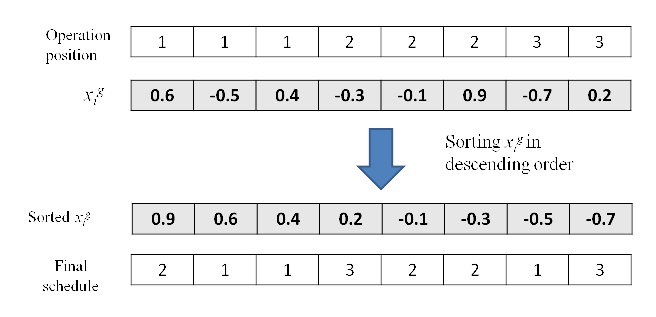
\includegraphics[width=\columnwidth]{./figures/deco.eps}
    \caption{Example of the decoding process used by the DE to solve FJSSP.}
    \label{fig:decodificacion}
    \vspace{-0.4cm}
\end{figure} 

\section{Our proposal: DE for FJSSP}
\label{sec:HDE}
\vspace{-0.2cm}
This section details our proposal to solve FJSSP. To apply the DE algorithm, it is crucial to design a suitable encoding scheme that map real-valued vectors to a feasible solution for FJSSP (see Section~\ref{subsec:rep}). Moreover, our proposal is enhanced by a simple local search (Section~\ref{subsec:HDE}). Finally, a parallel version of our proposal is introduced in Section~\ref{subsec:parallelHDE}.


\subsection{Representation}  \label{subsec:rep}

In this work, we adopt a random key encoding scheme~\cite{Bean1994RepRandomKeys}, which was used early with genetic algorithms for sequencing and optimization problems. It is based on random real numbers in a continuous space to encode solutions in a combinatorial space. In this way, the DE algorithm manipulates a real-valued vector to maintain the simplicity and properties in their natural configuration.

For a $n$-job $m$-machine scheduling problem, each vector's position (a random key) is a real number in U(-1,1). After a descending order of the random keys, the vector can be translated to a unique list of ordered operations. This procedure always obtains a feasible schedule, which is a permutation with repetitions~\cite{bierwirth1995}. 

Figure~\ref{fig:decodificacion} presents an example of the decoding process considering the instance shown in Table~\ref{tab:proccesingTime}. A fixed ID for each operation is first given following the job number and operation order within the job (represented as an operation position). The order of occurrence for each operation in the final schedule indicates its scheduling priority. Given the vector $x_i^g$=[0.6,-0.5,0.4,-0.3,-0.1,0.9,-0.7,0.2]. The last one is converted to the schedule $[2, 1, 1, 3, 2, 2, 1, 3]$, which is a permutation of the set of operations that represents a tentative ordering to schedule them, each one being represented by its ID number. This valid schedule corresponds to the operation sequence $O_{21}$, $O_{11}$, $O_{12}$, $O_{31}$, $O_{22}$, $O_{23}$, $O_{13}$, and $O_{32}$. 

In order to evaluate $x_i^g$, the objective value is the makespan or $C_{max}$ value. To compute it, each operation $O_{ij}$ in $x_i^g$ is assigned to a feasible machine $M_k$ in $U_{ij}$ with the shortest completion time, and then the load of $M_k$ must be updated. The initial solution is generated by a random procedure (Equation 1), mainly because high performing construction heuristics for FJSSP are unknown.

\subsection{DE and Local Search Method} \label{subsec:HDE}

DE is enhanced with a simple local search technique to improve the exploitation of promising regions of the search space. This new algorithm is called DE$_{LS}$. In this work, the local search method is a simple swap mechanism, which randomly selects two positions of the target vector and interchange its values. After that, a greedy selection takes place. If the modified solution presents an improvement in its $C_{max}$ value, then the swap is accepted, otherwise, it is discarded. The frequency of the local search is controlled by the probability $p_{LS}$. The pseudo-code of the local search procedure is given in Algorithm~\ref{alg:algoritmoLS}. 

This local search procedure is applied to the target vectors $x_{i}$ of the next population (just before Line 11 of Algorithm~\ref{alg:algoritmoDE}) but not to the trial vector $u_{i}$, which is beneficial to avoid both cycling search and getting trapped in a local optimum.  Another important feature of this local search procedure is that it does not need a backward conversion because it is applied over the real-valued vector.

\begin{algorithm} [!tb]
\scriptsize
    \caption{Local Search Procedure} \label{alg:algoritmoLS} 
    \begin{algorithmic} [1]
        \For {each $x_{i}^g$ from $P^{g}$}
            \If {$random() < p_{LS}$} %\Comment PBL: probabilidad de busqueda local
                \State $j$ , $k \leftarrow $ random(1,$D$)
                \State $u_{i} \leftarrow $ swap($x_{i}$, $j$,$k$)
                \If {$f(u_{i}) \leq  f(x_{i})$} \Comment{for a minimization problem}
                    \State $x_{i} \leftarrow u_{i}$
                \EndIf
            \EndIf
        \EndFor
    \end{algorithmic}
\end{algorithm}

\subsection{DE and Parallelism} \label{subsec:parallelHDE}
\vspace{-0.2cm}
In terms of designing parallel metaheuristics, the DE can be parallelized in different ways~\cite{Talbi}. In this work, the aim of the parallelization is not to change the behavior of the metaheuristic but to speed up the search. For that purpose, we focus on the parallelization of each iteration of the DE~\cite{albaPEA2006}. The population is decomposed and handled in parallel, using the well-known global parallelization model. The main process performs the selection operation, which is generally sequential. The rest processes (workers) perform the mutation, the recombination, and the evaluation of the solutions in parallel. Consequently, this model maintains the sequence of the original algorithm, and hence the behavior of the metaheuristic is not altered.

The local search method follows the same parallelization approach as previously mentioned. The solutions are assigned to different partitions, which are improved in parallel.
